\documentclass{article}
%Gummi|065|=)

\usepackage{graphicx}
\title{\textbf{Practica 3}}
\author{Omar Errandi}
\date{}
\begin{document}

\maketitle

\section{Define the TM solution of exercise 3.4 of the problem list and test its correct
behaviour.}
El enunciado del problema es el siguiente:

3.4. Prove that the function add(x,y) =x+y, withx,y∈N is Turing-computable using the unary notation \{ $|$ \}.  You have to create a TM with two arguments separated by a blank symbol that stars and ends behind the strings.

Para resolver el idea debemos de plantear unas reglas para nuestra maquina de Turing. La idea es rellenar el símbolo vacío que separa las cadenas y restar un $|$ para asi obtener nuestro resultado.



\centering
	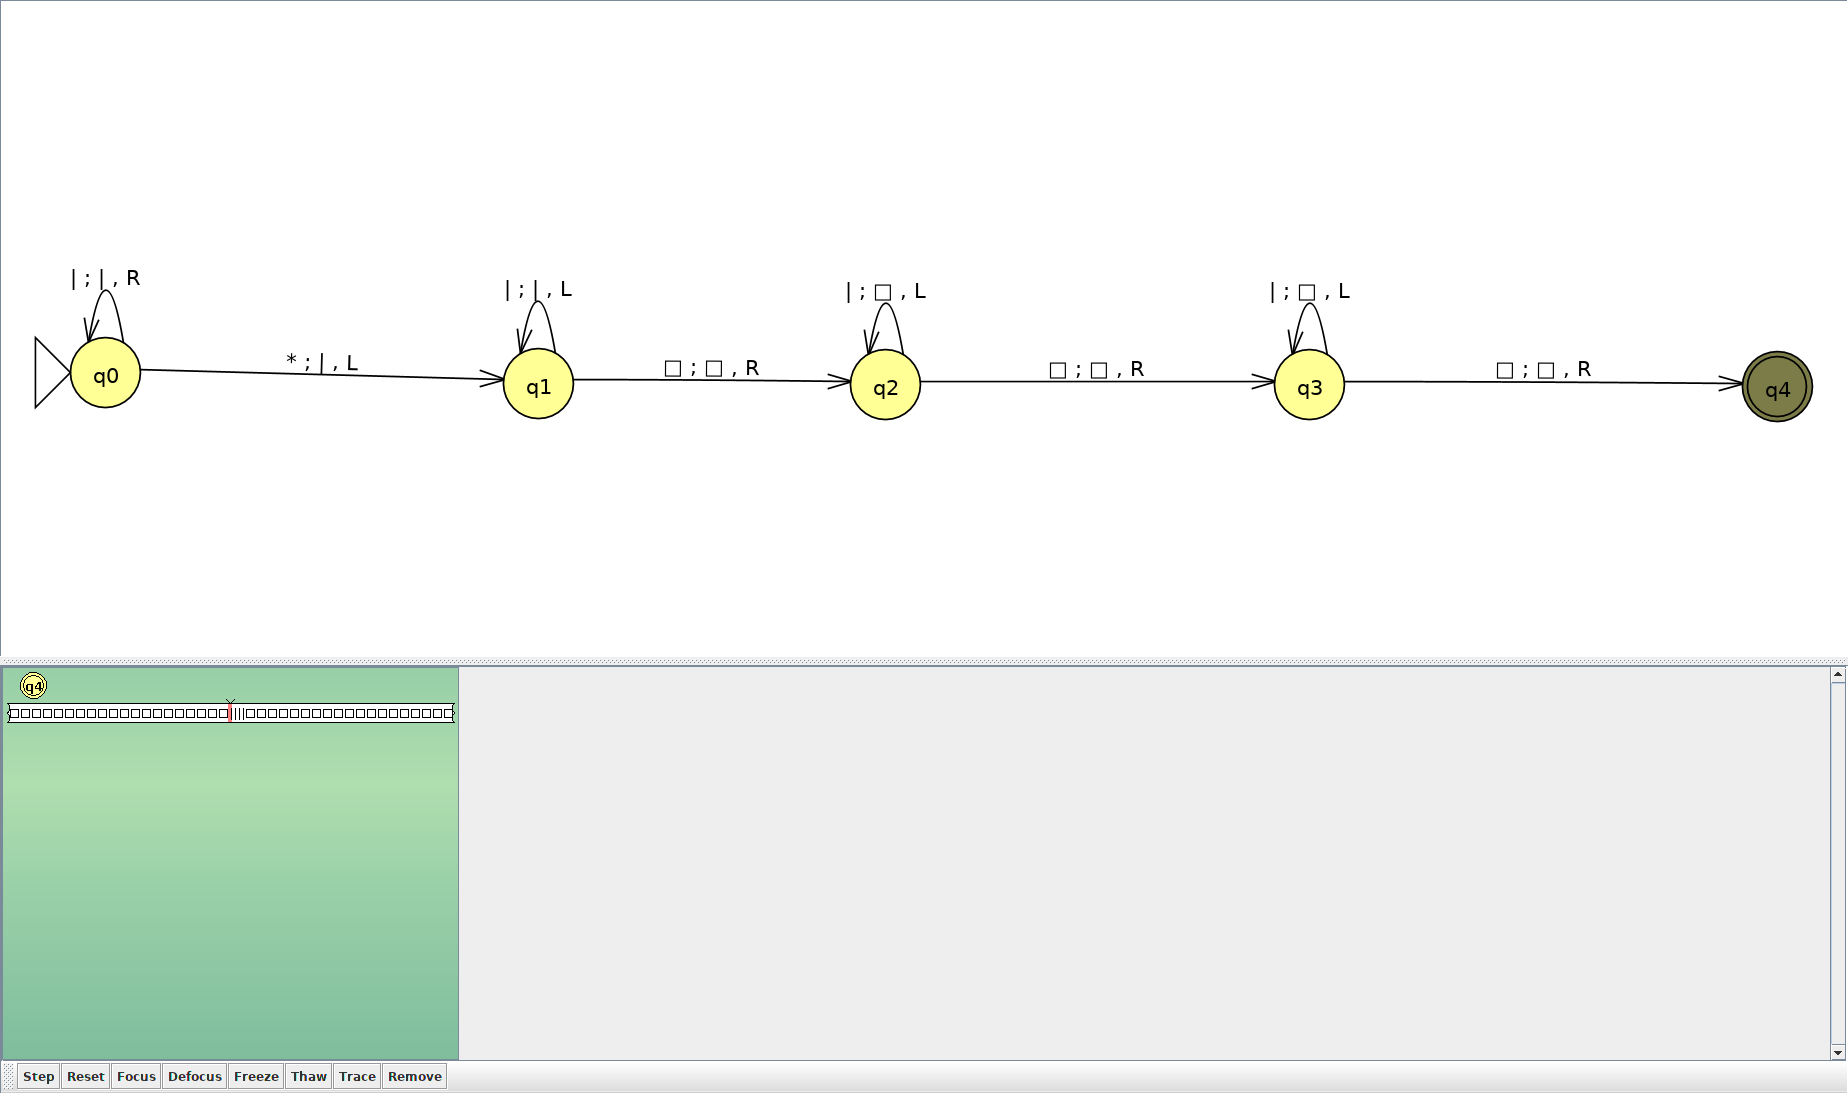
\includegraphics[scale=0.2]{Turing}
	\flushleft

Observamos que dandole como entrada la cadena $"||*|"$ el resultado que nos da es el correcto que es $"||||"$.

\section{Define a recursive function for the sum of three values.}
Primero de todo representamos la expresión de suma:

suma(x,y) = $\Biggl\{$$\begin{array}{ll}
		 \pi^1_{1}      & \mathrm{si\ } y = 0 \\
		 \sigma (\pi^3_{3}(x,y-1,suma({x,y-1}))) & \mathrm{si\ }  y> 0 \\
		 
	       \end{array}$
	       
	       
Por lo tanto a partir de la siguiente formula podemos deducir la operacion suma de tres valores:


sumaT(x,y,z) = $\Biggl\{$$\begin{array}{ll}
		 suma(x, y-1)      & \mathrm{si\ } z = 0 \\
		 \sigma (\pi^4_{4}(x,y,z-1,sumaT({x,y, z-1}))) & \mathrm{si\ }  z> 0 \\
		 
	       \end{array}$
	       
	      
Podemos testear nuestro codgo en Octave introduciendo lo siguiente:
\emph evalrecfunction($'<<\pi^1_1|\sigma(\pi^3_3)>|\sigma(\pi^4_4)>', (2,2,4$))

Y obtenemos:


\centering
	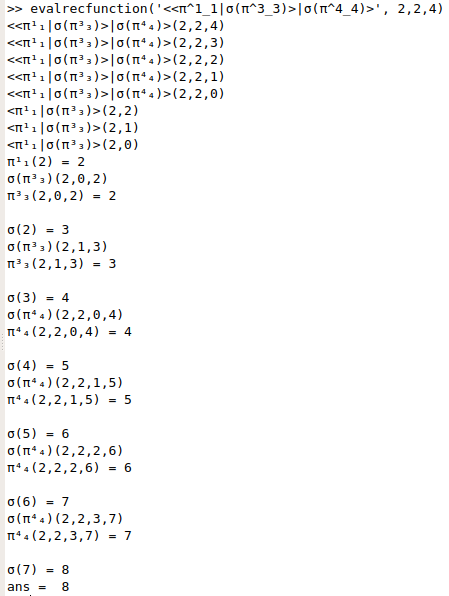
\includegraphics[scale=0.8]{imgOctave}
	\flushleft





\section{ Implement  a  WHILE  program  that  computes  the  sum  of  three  values.   You
must use an auxiliary variable that accumulates the result of the sum.}

Implementacion de sumaT:


  $X_4 := X_1\;$
  
  \textbf {while} $X_2$ != 0 \textbf {do}
  
  $X_4 := X_1 +1\;$
  $X_2 := X_2 -1\;$
  
  \textbf {od}
  
  \textbf {while} $X_3$ != 0 \textbf {do}
  
   $X_4 := X_1 +1\;$
  $X_3 := X_3 -1\;$
  
  \textbf {od}
 
  $X_1 := X_4\;$
 





\end{document}
